% ===== Page 47 =====
\origpage{47}
\subsection{General Procedure and the Fundamental Theorem}\label{ss:procedure}

\begin{itemize}[leftmargin=1.5em]
\item If $b\in\Range(A)$: \key{$\exists$ an exact solution} to $A\hat{x}=b$.
\item If $b\notin\Range(A)$:
\[
b_1=\operatorname{Proj}_{\Range(A)} b, \qquad A\hat{x}=b_1
\]
\begin{itemize}
\item If $\Null(A)=\{0\}$ $\Rightarrow$ \key{$\hat{x}$ is unique}.
\item If $\Null(A)\neq\{0\}$ $\Rightarrow$ $\hat{x}_1=\operatorname{Proj}_{\Null^\perp(A)}\hat{x}$
\end{itemize}
\end{itemize}

\begin{center}
\begin{tabular}{@{}l@{\quad}l@{}}
$\hat{x}$: & \term{minimum error solution} (least squares)\\
$\hat{x}_1$: & \term{minimum error-norm solution}
\end{tabular}
\end{center}

\begin{insight}[Why the procedure works]
\begin{itemize}[nosep,leftmargin=1.2em]
\item The error $b-A\hat x$ is smallest when $A\hat x$ is the point of $\Range(A)$ closest to $b$, i.e.\ $A\hat x=b_1=\operatorname{Proj}_{\Range(A)}b$ (orthogonality principle: $b-b_1\perp\Range(A)$). Writing this as $A\Hm(b-A\hat x)=0$ gives the \term{normal equations} $A\Hm A\hat x=A\Hm b$.
\item If $\Null(A)\neq\{0\}$, every $\hat x+n$ with $n\in\Null(A)$ gives the same $A\hat x=b_1$, so the least-squares solution is not unique. Splitting $\hat x=\hat x_1+\hat x_2$ with $\hat x_1\in\Null^\perp(A)$, $\hat x_2\in\Null(A)$ gives $A\hat x_1=A\hat x=b_1$ and, by Pythagoras, $\norm{\hat x+n}^2=\norm{\hat x_1}^2+\norm{\hat x_2+n}^2\geq\norm{\hat x_1}^2$. Hence \key{$\hat x_1$ is the least-squares solution of minimum norm}, and it does not depend on which $\hat x$ we started from.
\end{itemize}
\end{insight}

\begin{example}
$A=\bmat{1&2&3\\1&2&3}$, \qquad $n=3$, $m=2$ \quad ($A\in\C^{m\times n}$: $n$ columns, $m$ rows).
\begin{align*}
\Range(A)&=\Span\left\{\bmat{1\\1}\right\}, \qquad \dim(\Range(A))=1\\
\Null(A)&=\Span\left\{\bmat{3\\0\\-1},\bmat{2\\-1\\0}\right\}
\end{align*}
\[
\underbrace{\dim(\Range(A))}_{1}+\underbrace{\dim(\Null(A))}_{2}=3,
\qquad
\underbrace{\dim(\Null(A))}_{2}+\underbrace{\dim(\Null^\perp(A))}_{1}=3
\]
For $\Null^\perp(A)$, a vector $[a\ b\ c]\T$ orthogonal to both basis vectors of $\Null(A)$:
\[
\begin{aligned}3a-c&=0\\2a-b&=0\end{aligned}
\quad\Rightarrow\quad
\begin{aligned}c&=3a\\b&=2a\end{aligned}
\quad\Rightarrow\quad \bmat{a\\b\\c}=a\underbrace{\bmat{1\\2\\3}}_{\text{row of }A}
\qquad\Rightarrow\qquad
\Null^\perp(A)=\Span\left\{\bmat{1\\2\\3}\right\}
\]
\[
\Null^\perp(A)=\Range(A\Hm)
\]
\explain{$\therefore$ \key{Fundamental theorem of linear algebra.}}
\[
\hat{x}_1=\operatorname{Proj}_{\Null^\perp(A)}\hat{x}
=\operatorname{Proj}_{\Range(A\Hm)}\hat{x}
\]
\explain{$\Range(A\Hm)$: row space of $A$.}
\end{example}

\paragraph{Dimensions and rank.} For $A\in\C^{m\times n}$:
\begin{align*}
\dim(\underbrace{\Range(A)}_{k})+\dim(\underbrace{\Null(A)}_{n-k}) &= \#\text{ of columns}=n\\
\dim(\underbrace{\Null(A)}_{n-k})+\dim(\underbrace{\Range(A\Hm)}_{k})&=n
\qquad \big(\dim(\Null(A))+\dim(\Null^\perp(A))=n\big)
\end{align*}
\[
\left.\begin{aligned}
\dim(\Range(A))&=\#\text{ of lin.\ indep.\ columns of }A=\text{column rank}=k\\
\dim(\Range(A\Hm))&=\#\text{ of lin.\ indep.\ rows of }A=\text{row rank}=k
\end{aligned}\right\}\ k=\text{\term{rank} of a matrix}
\]
\[
\#\text{ linearly indep.\ rows}=\#\text{ linearly indep.\ columns}
\quad\text{as}\quad \dim\Range(A)=k=\dim\Range(A\Hm)
\]
$k$: \key{\# of linearly indep.\ rows $=$ \# of linearly indep.\ columns} (column rank $=$ row rank).

% ===== Page 48 =====
\origpage{48}
\begin{theorem}[Fundamental theorem of linear algebra]
$\Range(A\Hm)=\Null^\perp(A)$
\end{theorem}
\begin{proof}
$\inner{x}{y}\triangleq y\Hm x$.
\[
\inner{\underset{\C^m}{Ax}}{\underset{\C^m}{y}}_{\C^m}=y\Hm Ax=(A\Hm y)\Hm x=\inner{\underset{\C^n}{x}}{\underset{\C^n}{A\Hm y}}_{\C^n}
\]
Prove $\Null(A)=\Range^\perp(A\Hm)$, which is easier to prove.
\[
\left.\begin{aligned}
\Null(A)&\subset\Range^\perp(A\Hm)\\
\Range^\perp(A\Hm)&\subset\Null(A)
\end{aligned}\right\}\ \text{prove both}\ \Rightarrow\ \Null(A)=\Range^\perp(A\Hm)
\]

\paragraph{Part 1:} $x\in\Null(A)\Rightarrow Ax=0$.

\begin{minipage}{0.25\textwidth}
\centering
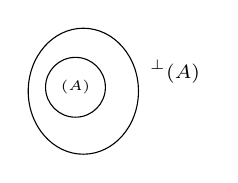
\begin{tikzpicture}
\draw (0,0) ellipse (0.7 and 0.8);
\draw (-0.1,0.05) circle (0.38);
\node[font=\tiny] at (-0.1,0.05) {$\Null(A)$};
\node[font=\scriptsize,anchor=west] at (0.72,0.25) {$\Range^\perp(A\Hm)$};
\end{tikzpicture}
\end{minipage}\hfill
\begin{minipage}{0.72\textwidth}
\begin{align*}
&\inner{Ax}{y}\quad\text{where }\forall y\in\C^m\\
&\inner{Ax}{y}=0\\
&\inner{x}{A\Hm y}=0\quad\forall y\in\C^m\\
\Rightarrow\ & x\perp A\Hm y\quad\forall y\in\C^m\\
\Rightarrow\ & x\perp\Range(A\Hm)\Rightarrow x\in\Range^\perp(A\Hm)
\end{align*}
\end{minipage}

\paragraph{Part 2:} $x\in\Range^\perp(A\Hm)$.

\begin{minipage}{0.25\textwidth}
\centering
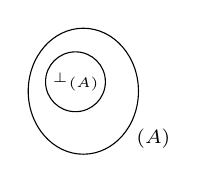
\begin{tikzpicture}
\draw (0,0) ellipse (0.7 and 0.8);
\draw (-0.1,0.12) circle (0.38);
\node[font=\tiny] at (-0.1,0.12) {$\Range^\perp(A\Hm)$};
\node[font=\scriptsize,anchor=west] at (0.55,-0.6) {$\Null(A)$};
\end{tikzpicture}
\end{minipage}\hfill
\begin{minipage}{0.72\textwidth}
\begin{align*}
&x\in\Range^\perp(A\Hm)\\
\Rightarrow\ & x\perp A\Hm y\quad\forall y\in\C^m\\
&\inner{x}{A\Hm y}=0\quad\forall y\in\C^m\\
&\inner{Ax}{y}=0\quad\forall y\in\C^m
\end{align*}
\explain{$Ax\in\C^m$, so choose $y=Ax$:}
\[
\inner{Ax}{Ax}=\norm{Ax}^2=0\Rightarrow Ax=0\Rightarrow x\in\Null(A)
\]
\end{minipage}

Both inclusions hold, so $\Null(A)=\Range^\perp(A\Hm)$. Taking orthogonal complements of both sides (in finite dimensions $(S^\perp)^\perp=S$ for a subspace $S$) gives $\Null^\perp(A)=\Range(A\Hm)$.
\end{proof}

\begin{center}
\begin{minipage}{0.46\textwidth}
\centering
\begin{tikzpicture}[scale=0.85]
\draw (0,0) ellipse (1.1 and 1.25);
\draw (0.05,0.15) ellipse (0.6 and 0.8);
\node[font=\scriptsize] at (0.05,-0.85) {$\Null(A)$};
\node at (0.9,-1.45) {$\C^n$};
\draw (3.8,0) ellipse (1.0 and 1.25);
\draw (3.75,0.15) ellipse (0.6 and 0.8);
\node[font=\scriptsize] at (3.75,-0.85) {$\Range(A)$};
\node at (4.75,-1.45) {$\C^m$};
\fill (3.55,0.45) circle (1.2pt) node[right,font=\scriptsize]{$0$};
\draw[-{Stealth[length=1.5mm]}] (-0.3,0.55) to[bend left=6] (3.5,0.47);
\draw[-{Stealth[length=1.5mm]}] (-0.25,0.25) to[bend left=3] (3.5,0.45);
\draw[-{Stealth[length=1.5mm]}] (-0.2,0.0) to[bend right=4] (3.5,0.43);
\draw[-{Stealth[length=2mm]}] (0.3,1.5) to[bend left=15] node[above]{$A$} (3.4,1.45);
\end{tikzpicture}
\end{minipage}\hfill
\begin{minipage}{0.5\textwidth}
\begin{align*}
&\dim(\overset{k}{\Range(A)})+\dim(\overset{n-k}{\Null(A)})=n\\
&\dim(\Null(A))+\dim(\Null^\perp(A))=n\\
&\underbrace{\dim(\Range(A\Hm))}_{k}+\underbrace{\dim(\Null(A))}_{n-k}=n\\
&\underbrace{\dim(\Range(A))}_{\text{column rank}}=\underbrace{\dim(\Range(A\Hm))}_{\text{row rank}}=k
\end{align*}
\explain{$k$: rank.}
\end{minipage}
\end{center}

\par\vskip 0pt plus 10\baselineskip\penalty-250\vskip 0pt plus -10\baselineskip
\subsection{Special Cases by Rank}\label{ss:rank-cases}
\subsubsection{Case I: Full Column Rank}
$A$ is/has \term{full column rank}: columns of $A$ are linearly independent.
\[
m\Big\{\underbrace{\overset{n}{\bmat{\ &\ &\ \\ \ &\ &\ \\ \ &\ &\ }}}_{\text{tall matrix}}
\overset{n}{\bmat{\ \\ \ \\ \ }}=\bmat{\ \\ \ \\ \ }\Big\}m \qquad m\geq n
\]
\begin{itemize}[nosep,leftmargin=1.5em]
\item $n=\#$ of unknowns, \quad $m=\#$ of equations
\item $m>n$: \term{overdetermined} system of eqn.
\end{itemize}
Assume
\[
\bmat{a&b&c\\d&e&f}\qquad\text{3 vectors cannot be linearly indep.\ for }\R^2.
\]
\explain{Under the columns: ``2 dim'', ``2 dimension''. Each column lies in $\R^2$, so at most $2$ of them can be linearly independent; full column rank therefore forces $m\geq n$.}

% ===== Page 49 =====
\origpage{49}
\begin{align*}
&\dim(\Range(A))=n\\
&\dim(\Null(A))=0\Rightarrow \Null(A)=\{0\} \qquad A\text{ is one-to-one}
\end{align*}
\key{If we have an exact solution, then the solution is unique.}

If $b\notin\Range(A)$:
\begin{align*}
P_{\Range(A)}&=B(B\Hm B)^{-1}B\Hm\\
\intertext{with $B=A$:}
P_{\Range(A)}&=A(A\Hm A)^{-1}A\Hm\\
b_1=P_{\Range(A)}b&=A(A\Hm A)^{-1}A\Hm b \qquad (A\hat{x}=b_1)\\
\Rightarrow\quad A\big(\underbrace{\hat{x}-(A\Hm A)^{-1}A\Hm b}_{\in\Null(A)}\big)&=0\\
\Rightarrow\quad \hat{x}-(A\Hm A)^{-1}A\Hm b&=0
\ \Rightarrow\ \boxed{\hat{x}=(A\Hm A)^{-1}A\Hm b}
\end{align*}
\explain{Unique solution as $\Null(A)=\{0\}$.}
$(A\Hm A)^{-1}A\Hm$: \term{left pseudo inverse} of $A$.

\begin{insight}
\begin{itemize}[nosep,leftmargin=1.2em]
\item \key{$A\Hm A$ ($n\times n$) is invertible exactly when $A$ has full column rank}: $A\Hm Ax=0\Rightarrow x\Hm A\Hm Ax=\norm{Ax}^2=0\Rightarrow Ax=0\Rightarrow x=0$.
\item The same formula comes directly from the normal equations $A\Hm A\hat x=A\Hm b$.
\item ``Left'' inverse: $\big((A\Hm A)^{-1}A\Hm\big)A=I_n$. If $b\in\Range(A)$, it returns the exact solution.
\end{itemize}
\end{insight}

\subsubsection{Case II: Full Row Rank}
$A$ is/has \term{full row rank}: all rows of $A$ are linearly indep.
\[
m\Big\{\underbrace{\overset{n}{\bmat{\ &\ &\ &\ \\ \ &\ &\ &\ }}}_{\text{fat matrix}}
\bmat{\ \\ \ \\ \ \\ \ }=\bmat{\ \\ \ } \qquad m\leq n
\]
\begin{itemize}[nosep,leftmargin=1.5em]
\item $m$: \# of equations, \quad $n$: \# of unknowns
\item $m<n$: \term{underdetermined} system of eqn.
\end{itemize}
\begin{align*}
\dim(\Range(A\Hm))&=m\\
\dim(\Range(A))&=m \ \Rightarrow\ \Range(A)=\C^m
\end{align*}
\[
b\in\Range(A)\quad\forall b\in\C^m\Rightarrow\text{\key{Always has an exact solution} (at least one): $A$ is onto.}
% corrected: notes had "b in C^m  for all b in R(A)" (quantifiers swapped)
\]
\begin{align*}
\hat{x}_1&=\operatorname{Proj}_{\Null^\perp(A)}\hat{x}=\operatorname{Proj}_{\Range(A\Hm)}\hat{x}\\
% corrected: notes had Proj_{R(A^H)} x-hat = Proj_{R(A^H)} x-hat (first projection meant onto N^perp(A))
\intertext{with $B=A\Hm$:}
P_{\Range(A\Hm)}&=A\Hm(AA\Hm)^{-1}A\\
\hat{x}_1&=A\Hm(AA\Hm)^{-1}\underbrace{A\hat{x}}_{b}\ \Rightarrow\ \hat{x}_1=A\Hm(AA\Hm)^{-1}b
\end{align*}
$A\Hm(AA\Hm)^{-1}$: \term{right pseudo inverse} of $A$.

\begin{insight}
\begin{itemize}[nosep,leftmargin=1.2em]
\item $AA\Hm$ ($m\times m$) is invertible since the rows of $A$ are independent (same argument as for $A\Hm A$, applied to $A\Hm$).
\item ``Right'' inverse: $A\big(A\Hm(AA\Hm)^{-1}\big)=I_m$, so $A\hat x_1=b$ is indeed an exact solution.
\item $\hat x_1=A\Hm\big((AA\Hm)^{-1}b\big)\in\Range(A\Hm)=\Null^\perp(A)$, so \key{it is the minimum-norm one} among the infinitely many exact solutions $\hat x_1+\Null(A)$.
\end{itemize}
\end{insight}

\subsubsection{Case III: Full Column and Full Row Rank}
$A$ is/has both full column and row rank.
\[
\left.\begin{aligned}m&\geq n\\ n&\geq m\end{aligned}\right\}\ m=n:\quad
\begin{aligned}
&A\text{ is a square matrix}\\
&\left.\begin{aligned}&A\text{ is one-to-one}\\&A\text{ is onto}\end{aligned}\right\}
\ \begin{aligned}&A\text{ has an inverse}\\&A\text{ is invertible.}\end{aligned}
\end{aligned}
\]
\explain{Both pseudo inverses reduce to $A^{-1}$ here: $(A\Hm A)^{-1}A\Hm=A^{-1}(A\Hm)^{-1}A\Hm=A^{-1}$ and $A\Hm(AA\Hm)^{-1}=A^{-1}$.}
\key{Exact solution exists. The solution is unique.}
\[
Ax=b,\qquad x_1=\hat{x}=x=A^{-1}b
\]

% ===== Page 50 =====
\origpage{50}
\begin{example}
\[
\underset{A}{\bmat{1&2\\1&2}}\underset{x}{\bmat{x_1\\x_2}}=\underset{b}{\bmat{1\\1}},
\qquad
\Range(A)=\Span\left\{\bmat{1\\1}\right\},\quad b\in\Range(A)
\ \Rightarrow\ \text{has exact solution},\quad \hat{x}=\bmat{1\\0}
\]

\begin{minipage}[c]{0.52\textwidth}
\begin{align*}
&\dim\Range(A)=1\\
&\dim\Null(A)=1\\
&\Null(A)=\Span\left\{\bmat{-2\\1}\right\}\\
&\hat{x}+n=\bmat{1\\0}+\alpha\bmat{-2\\1},\quad n\in\Null(A)
% corrected: notes had "x-hat + m" (an element of N(A) is added)
\end{align*}
\explain{In the sketch: $\Range(A\Hm)=\Span\{[1\ 2]\T\}$; the solution set $\hat x+\Null(A)$ is the line through $\hat x=[1\ 0]\T$ parallel to $\Null(A)$; $\hat{x}_1=\tfrac15[1\ 2]\T$ is its point on $\Range(A\Hm)$, and $\hat{x}_2=\hat x-\hat x_1\in\Null(A)$ is the part to ``get rid of''.}
\end{minipage}\hfill
\begin{minipage}[c]{0.44\textwidth}
\centering
\begin{tikzpicture}[scale=0.9,>={Stealth[length=1.6mm]}]
\draw[->] (-2.5,0)--(2.7,0) node[right]{$x_1$};
\draw[->] (0,-1.7)--(0,2.2) node[above]{$x_2$};
% R(A^H): y = 2x
\draw[very thick,blue!50!black] (-0.85,-1.7)--(1.05,2.1) node[above right,font=\scriptsize]{$\Range(A\Hm)$};
% N(A): y = -x/2 through origin
\draw (-2.5,1.25)--(2.7,-1.35) node[below,font=\scriptsize]{$\Null(A)$};
% solution set: through (1,0), slope -1/2
\draw[gray!70!black] (-1.8,1.4)--(2.7,-0.85) node[right,font=\scriptsize]{$\hat x+\Null(A)$};
% ticks
\foreach \t in {-2,1,2} \draw (\t,0.06)--(\t,-0.06);
\node[font=\tiny,below] at (-2,0) {$-2$};
\node[font=\tiny,above] at (2,0) {$2$};
\node[font=\tiny,above right] at (1,0) {$1$};
\draw[dashed,gray] (-2,0)--(-2,1)--(0,1);
\draw[dashed,gray] (2,0)--(2,-1)--(0,-1);
% right angle at x1hat
\draw ($(0.2,0.4)+(-0.0894,-0.1789)$) -- ++(0.1789,-0.0894) -- ++(0.0894,0.1789);
\fill (0.2,0.4) circle (1.4pt);
\node[font=\scriptsize,left] at (0.05,0.55) {$\hat{x}_1$};
\fill (1,0) circle (1.4pt);
\node[font=\scriptsize,below] at (1.1,0) {$\hat{x}$};
\draw[->,dashed,thick] (0,0)--(0.8,-0.4) node[font=\scriptsize,below]{$\hat{x}_2$};
\end{tikzpicture}
\end{minipage}

\explain{Check: $\hat x_1=\tfrac15\bmat{1\\2}$ gives $A\hat x_1=\bmat{1\\1}=b$, and $\norm{\hat x_1}^2=\tfrac15<1=\norm{\hat x}^2$; the right pseudo inverse cannot be used here since $AA\Hm=\bmat{5&5\\5&5}$ is singular ($A$ has rank 1, neither full row nor full column rank), so the projection route is used.}
\end{example}

\subsubsection{Case IV: Neither Full Column nor Full Row Rank}
$A$ is/has neither full column rank nor full row rank.

\begin{example}
\[
\underset{A}{\bmat{1&0&1\\1&1&2\\0&1&1}}\underset{x}{\bmat{x_1\\x_2\\x_3}}=\underset{b}{\bmat{1\\0\\3}}
\qquad
\begin{aligned}
&2\text{ linearly indep.\ columns}\\
&2\text{ linearly indep.\ rows}\\
&\dim(\Range(A))=\dim(\Range(A\Hm))=2\\
&\dim(\Null(A))=1\\
&\dim(\Null^\perp(A))=2
\end{aligned}
\]
\[
\bmat{1\\0\\3}=\underset{\alpha}{\underset{\parallel}{1}}\bmat{1\\1\\0}+\underset{\beta}{\underset{\parallel}{3}}\bmat{0\\1\\1}\quad\times
\qquad\Rightarrow\qquad b\notin\Range(A)\Rightarrow\text{\key{No exact solution.}}
\]
\explain{Column 3 $=$ column 1 $+$ column 2, so $\Range(A)=\Span\{[1\ 1\ 0]\T,[0\ 1\ 1]\T\}$. Matching the 1st and 3rd entries of $b$ forces $\alpha=1$, $\beta=3$, but then the 2nd entry would be $\alpha+\beta=4\neq0$.}

\paragraph{Method I.}
\begin{align*}
P_{\Range(A)}&=B(B\Hm B)^{-1}B\Hm\\
B&=\bmat{1&0\\1&1\\0&1},\qquad B\Hm B=\bmat{1&1&0\\0&1&1}\bmat{1&0\\1&1\\0&1}=\bmat{2&1\\1&2}\\
(B\Hm B)^{-1}&=\frac13\bmat{2&-1\\-1&2}\\
P_{\Range(A)}&=\bmat{1&0\\1&1\\0&1}\frac13\bmat{2&-1\\-1&2}\bmat{1&1&0\\0&1&1}=\frac13\bmat{2&1&-1\\1&2&1\\-1&1&2}\\
b_1=P_{\Range(A)}b&=\frac13\bmat{-1\\4\\5}
\end{align*}
\[
\underbrace{\bmat{1&0&1\\1&1&2\\0&1&1}}_{A}\underbrace{\bmat{x_1\\x_2\\x_3}}_{\hat{x}}=\underbrace{\frac13\bmat{-1\\4\\5}}_{b_1}
\qquad\Rightarrow\qquad \underset{\text{minimum error solution.}}{\hat{x}=\frac13\bmat{-1\\5\\0}}
\]
\explain{This was method I. With $x_3=0$: $x_1=-\tfrac13$, $x_1+x_2=\tfrac43\Rightarrow x_2=\tfrac53$, and the 3rd row $x_2+x_3=\tfrac53$ checks. The error is $b-b_1=\tfrac43[1\ {-1}\ 1]\T$, which is orthogonal to both columns of $B$, as it must be.}

\paragraph{Method II.}
\[
\underbrace{\bmat{1&0\\1&1\\0&1}}_{A_1}\underbrace{\bmat{x_1\\x_2}}_{z}=\bmat{1\\0\\3}
\qquad
\begin{aligned}
&\Rightarrow\Null(A_1)=\{0\}\\
&\Rightarrow\text{full column rank}\\
&\Rightarrow\text{Exact solution is known}
\end{aligned}
\]
% corrected: notes had z = [x2; x3]; A_1 consists of the first two columns of A, so z = [x1; x2] (consistent with the final x-hat).
\explain{Idea: drop the dependent third column (set $x_3=0$); the remaining $A_1$ has full column rank and $\Range(A_1)=\Range(A)$, so Case I applies.}
\[
\hat{z}=(A_1\Hm A_1)^{-1}A_1\Hm b=\frac13\bmat{2&-1\\-1&2}\bmat{1&1&0\\0&1&1}\bmat{1\\0\\3}=\underbrace{\frac13\bmat{-1\\5}}_{\hat{z}\ \to\ \text{unique}}
\qquad\therefore\ \hat{x}=\frac13\bmat{-1\\5\\0}
\]

% ===== Page 51 =====
\origpage{51}
\paragraph{Minimum norm solution.} $A\Hm=A\T$ as matrix is real.
\begin{align*}
A\Hm&=\bmat{1&1&0\\0&1&1\\1&2&1}\\
P_{\Range(A\Hm)}&=B(B\Hm B)^{-1}B\Hm,\qquad B=\bmat{1&0\\0&1\\1&1}\\
(B\Hm B)^{-1}&=\frac13\bmat{2&-1\\-1&2}\\
P_{\Range(A\Hm)}&=\frac13\bmat{2&-1&1\\-1&2&1\\1&1&2}\\
\hat{x}_1=P_{\Range(A\Hm)}\hat{x}&=\frac19\bmat{-7\\11\\4}
\end{align*}
\explain{$\therefore$ \key{$\hat{x}_1$: minimum error, minimum norm solution.}}
\begin{insight}[Check]
$A\hat x_1=\tfrac19[-3\ \ 12\ \ 15]\T=\tfrac13[-1\ \ 4\ \ 5]\T=b_1$, so $\hat x_1$ has the same (minimum) error as $\hat x$. Moreover $\hat x-\hat x_1=\tfrac49[1\ \ 1\ {-1}]\T$ spans $\Null(A)$ (indeed $A[1\ 1\ {-1}]\T=0$), and
$\norm{\hat x_1}^2=\tfrac{186}{81}\approx2.30<\tfrac{26}{9}\approx2.89=\norm{\hat x}^2$.
\end{insight}
\end{example}

\section{Spectral Analysis of Linear Transformations}\label{sec:spectral}
\syllabusweek{Weeks 8--9 --- eigenvalues and eigenvectors, invariance under operators, block diagonal forms}
\subsection{Invariant Subspaces}\label{ss:invariant}
\[
A\qquad \{\lambda_1,\lambda_2,\dots,\lambda_n\}:\ \text{\term{spectrum} of a matrix}
\]
\begin{definition}
Let $\mathcal{A}:\V\to\V$ be a linear transformation defined over a vector space $\V$. A subspace $M$ of $\V$ is said to be \term{invariant under $\mathcal{A}$} iff
\[
\mathcal{A}x\in M\quad\forall x\in M
\]
\end{definition}
\begin{center}
\begin{tikzpicture}
\draw (0,0) ellipse (0.8 and 0.9);
\draw (0.05,0.05) circle (0.42);
\node[font=\scriptsize] at (-0.45,0.62) {$M$};
\node[font=\scriptsize] at (0,-1.15) {$\V$};
\draw (3.2,0.1) ellipse (0.7 and 0.9);
\draw (3.2,0.15) circle (0.42);
\node[font=\scriptsize] at (3.2,0.78) {$M$};
\node[font=\scriptsize] at (3.85,-0.85) {$\V$};
\fill (-0.1,-0.05) circle (1pt);
\fill (3.1,0.2) circle (1pt);
\draw[-{Stealth[length=1.5mm]}] (-0.1,-0.05) -- node[above]{$\mathcal{A}$} (3.05,0.2);
\end{tikzpicture}
\end{center}

\begin{example}
$\V=\{f\mid f\text{ functions defined over }\R\text{ which are infinitely differentiable}\}$
\[
\mathcal{A}=\frac{d}{dt}:\ \V\to\V, \qquad M_1\triangleq\Span\{\sin t\}\subset\V
\]
\[
\mathcal{A}(\alpha\sin t)=\alpha\mathcal{A}\sin t=\alpha\cos t\notin M_1
\]
$\therefore$ \key{$M_1$ is not invariant under $\mathcal{A}$.}
\begin{align*}
M_2&\triangleq\Span\{\cos t,\sin t\}\\
x&=\alpha_1\cos t+\alpha_2\sin t\\
\mathcal{A}x&=-\alpha_1\sin t+\alpha_2\cos t\in\Span\{\cos t,\sin t\}= M_2
\end{align*}
$\therefore$ \key{$M_2$ is invariant under $\mathcal{A}$.}
\begin{align*}
M_3&=\{0\}, \qquad \mathcal{A}0=0\in M_3\\
M_4&=\Span\{e^{2t}\},\qquad x=\alpha e^{2t},\qquad \mathcal{A}x=2\alpha e^{2t}\in M_4
\end{align*}
$\therefore$ $M_3$ and $M_4$ are invariant under $\mathcal{A}$ ($e^{2t}$ is mapped to a multiple of itself: it is an ``eigenfunction'' of $\frac{d}{dt}$ with eigenvalue $2$).
\end{example}
% corrected: the notes write "not in M" for M_1; made explicit as M_1.
\begin{insight}
The trivial subspaces $\{0\}$ and $\V$ are always invariant. \key{A one-dimensional subspace $\Span\{e\}$ is invariant iff $\mathcal{A}e=\lambda e$} for some scalar $\lambda$, i.e.\ iff $e$ is an eigenvector --- this is the link between invariant subspaces and the eigenvalues defined below.
\end{insight}

% ===== Page 52 =====
\origpage{52}
\begin{example}
$\Null(\mathcal{A})$ \& $\Range(\mathcal{A})$ are invariant under $\mathcal{A}$.

\begin{minipage}[t]{0.48\textwidth}
\underline{$\Null(\mathcal{A})$:}\quad $x\in\Null(\mathcal{A})$
\[
\mathcal{A}x=0_{\V}\in\Null(\mathcal{A})
\]
$\Null(\mathcal{A})$ is invariant under $\mathcal{A}$.
\end{minipage}\hfill
\begin{minipage}[t]{0.48\textwidth}
\underline{$\Range(\mathcal{A})$:}\quad $x\in\Range(\mathcal{A})$
\[
\mathcal{A}x\in\Range(\mathcal{A})
\]
$\Range(\mathcal{A})$ is invariant under $\mathcal{A}$.
\end{minipage}
\end{example}

\subsection{Powers and Polynomials of a Linear Transformation}\label{ss:powers}
\begin{definition}
\term{Powers} of a linear transformation $\mathcal{A}:\V\to\V$ are defined as
\[
\mathcal{A}^k x=\underbrace{\mathcal{A}(\mathcal{A}\cdots\mathcal{A}(\mathcal{A}x)\dots)}_{\mathcal{A}\text{ is applied }k\text{ times}}
\]
\end{definition}
When domain and co-domains are the same, then we can define the power of a linear transformation.
\begin{itemize}[nosep,leftmargin=1.5em]
\item $\R^n\to\R^m$, $m\neq n$ $\Rightarrow$ not defined.
\item $\mathcal{A}:\V\to\W$: \ $\mathcal{A}(\underbrace{\mathcal{A}x}_{\in\W})$ \ $\times$ not defined, since $\mathcal{A}$ acts on elements $\in\V$.
\end{itemize}

\sep
$\star$ \term{Polynomials of $\mathcal{A}$} can be constructed using linear combinations of powers of $\mathcal{A}$.

\begin{minipage}{0.66\textwidth}
\begin{align*}
p(s)&=\alpha_0s^n+\alpha_1s^{n-1}+\dots+\alpha_{n-1}s+\alpha_n\,(s^0)\\
p(\mathcal{A})&=\alpha_0\mathcal{A}^n+\alpha_1\mathcal{A}^{n-1}+\dots+\alpha_{n-1}\mathcal{A}^1+\alpha_n\mathcal{A}^0\\
p(\mathcal{A})&=\alpha_0\mathcal{A}^n+\dots+\alpha_{n-1}\mathcal{A}+\alpha_nI
\end{align*}
\end{minipage}\hfill
\begin{minipage}{0.28\textwidth}
\begin{keybox}
\centering
$\mathcal{A}^0x=x=Ix$\\
$\mathcal{A}^0=I$
\end{keybox}
\end{minipage}

For example, with $p(\mathcal{A})=3\mathcal{A}^3+2\mathcal{A}^2+\mathcal{A}+I$:
\begin{align*}
p(\mathcal{A})\mathcal{A}x&=(3\mathcal{A}^3+2\mathcal{A}^2+\mathcal{A}+I)\mathcal{A}x=3\mathcal{A}^4x+2\mathcal{A}^3x+\mathcal{A}^2x+\mathcal{A}x\\
&=\mathcal{A}(3\mathcal{A}^3x+2\mathcal{A}^2x+\mathcal{A}x+x)\\
&=\mathcal{A}\underbrace{(3\mathcal{A}^3+2\mathcal{A}^2+\mathcal{A}+I)}_{p(\mathcal{A})}x
\end{align*}
\[
\boxed{p(\mathcal{A})\mathcal{A}x=\mathcal{A}p(\mathcal{A})x\quad\forall x\in\V}
\qquad\Rightarrow\qquad
p(\mathcal{A})\mathcal{A}=\mathcal{A}p(\mathcal{A})
\]
\explain{\key{$\mathcal{A}$ commutes with $p(\mathcal{A})$.}}

\begin{example}
$\Null(p(\mathcal{A}))$ \& $\Range(p(\mathcal{A}))$ are invariant under $\mathcal{A}$.

\underline{$\Null(p(\mathcal{A}))$:} \ $x\in\Null(p(\mathcal{A}))$. \ Is $\mathcal{A}x\in\Null(p(\mathcal{A}))$?
\begin{align*}
p(\mathcal{A})\mathcal{A}x&=\mathcal{A}\underbrace{p(\mathcal{A})x}_{0_{\V}}=\mathcal{A}0_{\V}=0_{\V}\\
&\Rightarrow\mathcal{A}x\in\Null(p(\mathcal{A}))
\end{align*}

% ===== Page 53 =====
\origpage{53}
\underline{$\Range(p(\mathcal{A}))$:} \ $x\in\Range(p(\mathcal{A}))$, \ $x=p(\mathcal{A})y$.
\begin{align*}
\mathcal{A}x&=\mathcal{A}p(\mathcal{A})y=p(\mathcal{A})\underbrace{\mathcal{A}y}_{y'}=p(\mathcal{A})y'\\
&\Rightarrow\mathcal{A}x\in\Range(p(\mathcal{A}))
\end{align*}
\end{example}

\subsection{Eigenvalues and Eigenvectors}\label{ss:eigen}
$\star$ Matrix representation:
\[
\mathcal{A}:\underset{\substack{\downarrow\\ B\\ \text{basis set}\\ \text{for }\V}}{\overset{n}{\V}}\to\underset{\substack{\downarrow\\ B\\ \text{basis set}\\ \text{for }\V}}{\overset{n}{\V}}
\qquad A:\C^n\to\C^n
\qquad
\begin{aligned}
y&=\mathcal{A}x &\quad \lambda e&=\mathcal{A}e\\
&\Downarrow & &\Downarrow\\
[y]_B&=A[x]_B & \lambda[e]_B&=A[e]_B
\end{aligned}
\]
\[
\det\mathcal{A}\triangleq\det A,\qquad \tr\mathcal{A}\triangleq\tr A
\]
% corrected: notes had "tr A := det A" (slip; the trace of the operator is the trace of its matrix)
\explain{Well defined: another basis gives $\bar A=P^{-1}AP$, and $\det(P^{-1}AP)=\det A$, $\tr(P^{-1}AP)=\tr A$.}

\begin{definition}
Let $A$ denote the matrix representation of a linear transformation $\mathcal{A}$ from $\V$ into $\V$ ($A$ is a square matrix). The \term{eigenvalues} of $\mathcal{A}$ denoted by $\lambda_i$ are defined as the $n$ roots of the equation
\[
\det(sI-A)=0,
\]
where $d(s)\triangleq\det(sI-A)$ is called the \term{characteristic polynomial} of $A$.
The vectors $e_i\neq0$ satisfying $Ae_i=\lambda_i e_i$ are called \term{eigenvectors} of $A$.
\end{definition}

\begin{center}
\begin{minipage}{0.48\textwidth}
\centering
\begin{tikzpicture}[scale=0.75,>={Stealth[length=1.8mm]}]
\draw (-3,0)--(3,0);
\draw[->] (0,-1.5)--(0,2.8);
\draw[->] (0,0)--(0.25,2.6) node[above right]{$\mathcal{A}x$};
\draw[->] (0,0)--(0.8,1.9) node[above]{$x$};
\draw[->] (0,0)--(2.6,1.3) node[above]{$2e_i$};
\draw[->,very thick] (0,0)--(1.3,0.65) node[below right]{$e_i$};
\draw[->] (0,0)--(-2.6,-1.3) node[below]{$-2e_i$};
\end{tikzpicture}
\end{minipage}\hfill
\begin{minipage}{0.45\textwidth}
\begin{align*}
&\mathcal{A}e_i=\lambda_ie_i\\
&\lambda_i=2\\
&\lambda_i=-2
\end{align*}
\explain{A general $x$ is turned into a different direction ($\mathcal{A}x\not\parallel x$); an eigenvector $e_i$ is only scaled, e.g.\ to $2e_i$ if $\lambda_i=2$ or to $-2e_i$ if $\lambda_i=-2$, so the line $\Span\{e_i\}$ is invariant.}
\end{minipage}
\end{center}

\sep
\[
A=\underset{\text{rotation matrix}}{\bmat{0&-1\\1&0}}\qquad
x_1=\bmat{1\\0}\qquad x_2=\bmat{0\\1}\qquad x_3=\bmat{1\\1}
\]

\begin{minipage}{0.42\textwidth}
\centering
\begin{tikzpicture}[scale=1.1,>={Stealth[length=1.8mm]}]
\draw[->] (-1.7,0)--(1.8,0);
\draw[->] (0,-1.0)--(0,1.6);
\draw[->,thick] (0,0)--(1,0) node[below]{$x_1$};
\draw[->] (-0.04,0)--(-0.04,1) node[above left,inner sep=1pt]{$x_2$};
\draw[->,very thick] (0.03,0)--(0.03,1) node[above right,inner sep=1pt]{$\mathcal{A}x_1$};
\draw[->] (0,0.03)--(-1,0.03) node[below]{$\mathcal{A}x_2$};
\draw[->] (0,0)--(1,1) node[right]{$x_3$};
\draw[->] (0,0)--(-1,1) node[left]{$\mathcal{A}x_3$};
\end{tikzpicture}
\end{minipage}\hfill
\begin{minipage}{0.55\textwidth}
\begin{align*}
&s^2+1=0\qquad\lambda_{1,2}=\mp j\\
&\underset{\text{real}}{A}e_i=\underset{\text{complex}}{\lambda_i}e_i\qquad R:\text{ rotation matrix}\\
&Re_i=\lambda_ie_i\\
&\norm{Re_i}=\norm{\lambda_ie_i}\\
&\cancel{\norm{e_i}}=\abs{\lambda_i}\cancel{\norm{e_i}}\qquad (e_i:\text{ nonzero vector})\\
&\abs{\lambda_i}=1\\
&\therefore\ \boxed{\lambda_i=e^{j\omega}}
\end{align*}
\end{minipage}
% corrected: notes had "R: rotation vectors"; R denotes the rotation matrix
\begin{insight}
No real vector keeps its direction under a $90^\circ$ rotation, so there are no real eigenvectors; the eigenvectors are complex: $A\bmat{1\\-j}=\bmat{j\\1}=j\bmat{1\\-j}$ and $A\bmat{1\\j}=-j\bmat{1\\j}$. A rotation preserves length, $\norm{Re}=\norm{e}$ (also for complex $e$, since $R\Hm R=I$), which is what forces $\abs{\lambda_i}=1$; here $\lambda=\pm j=e^{\pm j\pi/2}$, i.e.\ $\omega=\pm\pi/2$ is the rotation angle.
\end{insight}

% ===== Page 54 =====
\origpage{54}
\sep
$\star$ Existence of eigenvectors:
\[
A\overset{\neq0}{e_i}=\lambda e_i\qquad d(\lambda)=\det(\lambda_iI-A)=0
\]
\begin{align*}
&A=[c_1\ c_2\ \dots\ c_n]\\
&\exists\ \alpha_1,\alpha_2,\dots,\alpha_n\text{ not all equal to zero satisfying}\\
&\qquad\alpha_1c_1+\alpha_2c_2+\dots+\alpha_nc_n=0\\
&\qquad\underset{A}{[c_1\ c_2\ \dots\ c_n]}\bmat{\alpha_1\\\alpha_2\\\vdots\\\alpha_n}=0
\end{align*}
\explain{$A$ is not full column rank $\Rightarrow$ $\exists\alpha\neq0$ s.t.\ $A\alpha=0$. Apply this to the singular matrix $\lambda_iI-A$ ($\det(\lambda_iI-A)=0$ means its columns are dependent):}
\begin{align*}
&\exists\alpha\ \text{s.t.}\ (\lambda_iI-A)\alpha=0\\
&\qquad A\alpha=\lambda_i\alpha\ \Rightarrow\ \text{Eğer bir eigenvalue varsa en az 1 eigenvector vardır}
\end{align*}
\explain{\key{If there is an eigenvalue, then there is at least 1 eigenvector}: $\alpha\neq0$ is an eigenvector for $\lambda_i$.}

\begin{example}
\begin{align*}
A&=\bmat{2&1\\1&2},\qquad d(s)=\det(sI-A)=\det\bmat{s-2&-1\\-1&s-2}\\
&=(s-2)^2-1=s^2-4s+3=(s-3)(s-1)=0\\
&\Rightarrow\ \lambda_1=3,\quad\lambda_2=1
\end{align*}
\begin{align*}
&Ae_i=\lambda_ie_i\\
&(A-\lambda_iI)e_i=0\\
&e_i\in\underbrace{\Null(A-\lambda_iI)}_{\text{\term{eigenspace}}},\quad\dim\geq1
\qquad\qquad
\begin{aligned}
p(s)&=s-\lambda_i\\
p(A)&=A-\lambda_iI
\end{aligned}
\end{align*}
\begin{align*}
A-\lambda_1I&=\bmat{-1&1\\1&-1}, \qquad e_1=\bmat{1\\1}\\
A-\lambda_2I&=\bmat{1&1\\1&1}, \qquad\quad\ e_2=\bmat{1\\-1}
\end{align*}
\begin{align*}
\Null(A-\lambda_1I)&=\Span\left\{\bmat{1\\1}\right\}\\
\Null(A-\lambda_2I)&=\Span\left\{\bmat{1\\-1}\right\}
\end{align*}
\[
\Null(A-\lambda_1I)\overset{\perp}{\oplus}\Null(A-\lambda_2I)=\C^2
\]
% corrected/simplified: notes put perp marks over each N(.) and "dim = 2" marks over C^2
\explain{$\overset{\perp}{\oplus}$: basis vectors are linearly indep.\ and orthogonal ($[1\ 1]\T\perp[1\ {-1}]\T$); dimensions $1+1=2=\dim\C^2$.}
\[
\alpha\bmat{1\\1}+\beta\bmat{1\\-1}=\begin{matrix}\R^2\\\C^2\end{matrix}
\]
\[
\alpha\bmat{1\\1}+\beta\bmat{1\\-1}=\bmat{0\\0}\quad\text{iff }\alpha=\beta=0
\ \Rightarrow\ \text{subspaces are linearly indep.}
\]
\explain{Orthogonality is special here because $A=A\Hm$ is Hermitian; in general eigenspaces are only linearly independent (see p.~57).}
\end{example}

% ===== Page 55 =====
\origpage{55}
\sep
$\star$ Change of basis:
\[
y=Ax,\qquad B=\left\{\bmat{1\\0},\bmat{0\\1}\right\}\ \to\ \text{canonical basis set}
\]
\[
x=\bmat{x_1\\x_2},\quad [x]_B,\qquad [y]_B=A[x]_B\ \sim\ [y]_{\bar{B}}=\bar{A}[x]_{\bar{B}},
\qquad
\bmat{x_1\\x_2}=x_1\bmat{1\\0}+x_2\bmat{0\\1}
\]
\[
\bar{B}=\left\{\bmat{1\\1},\bmat{1\\-1}\right\},\qquad A=\bmat{2&1\\1&2}
\]
\begin{align*}
x&=\bmat{1\\1}, & [x]_{\bar{B}}&=\bmat{1\\0}, & y=Ax&=\bmat{3\\3}=3\bmat{1\\1}, & [y]_{\bar{B}}&=\bmat{3\\0}\\
&& \bmat{3\\0}&=\bar{A}\bmat{1\\0} & \Rightarrow\ \bar{A}&=\bmat{3&\\0&}\\[4pt]
x&=\bmat{1\\-1}, & [x]_{\bar{B}}&=\bmat{0\\1}, & y=Ax&=\bmat{1\\-1}=1\bmat{1\\-1}, & [y]_{\bar{B}}&=\bmat{0\\1}\\
&& \bmat{0\\1}&=\bar{A}\bmat{0\\1} & \Rightarrow\ \bar{A}&=\bmat{3&0\\0&1}
\end{align*}

\sep
\[
P=[e_1\mid e_2],\qquad \bar{A}=f(A)=\ ?
\]
\[
\begin{aligned}Ae_1&=\lambda_1e_1\\Ae_2&=\lambda_2e_2\end{aligned}
\]
\begin{align*}
[\lambda_1e_1,\lambda_2e_2]&=[Ae_1\mid Ae_2]=A[e_1\mid e_2]\\
\underbrace{[e_1\ e_2]}_{P}\underbrace{\bmat{\lambda_1&0\\0&\lambda_2}}_{\bar{A}}&=A\cdot P
\ \Rightarrow\ P\bar{A}=AP\\
&\Rightarrow\ \boxed{\bar{A}=P^{-1}AP}
\end{align*}
\explain{$P$ is invertible (full rank: its columns $e_1,e_2$ are linearly indep.).}
\begin{insight}
The columns of $P$ are the new basis vectors written in the old basis, so $[x]_B=P[x]_{\bar B}$. Then $[y]_B=A[x]_B$ becomes $P[y]_{\bar B}=AP[x]_{\bar B}$, i.e.\ $[y]_{\bar B}=P^{-1}AP\,[x]_{\bar B}$. Check: $P=\bmat{1&1\\1&-1}$, $P^{-1}=\tfrac12\bmat{1&1\\1&-1}$, $P^{-1}AP=\tfrac12\bmat{1&1\\1&-1}\bmat{3&1\\3&-1}=\bmat{3&0\\0&1}$, as found above.
\end{insight}
\[
\C^2=\underset{1}{\Null(A-\lambda_1I)}\overset{\perp}{\oplus}\underset{1}{\Null(A-\lambda_2I_2)},
\qquad
\left[\begin{array}{c|c}\overset{1\times1}{\lambda_1}&0\\\hline 0&\lambda_2\end{array}\right]
\]
\explain{Each block is $1\times1$ as $\dim\Null(A-\lambda_2I_2)=1$.}

\subsection{Block Diagonal Representations}\label{ss:block-diag}
\begin{theorem}[Block diagonal representation]
Consider the linear transformation
\[
y=Ax\quad\text{where }A\in\C^{n\times n},\ y,x\in\C^n.
\]
Suppose that
\begin{enumerate}[label=\roman*)]
\item $\C^n=M_1\oplus M_2\oplus\dots\oplus M_k$
\item $M_i$ is invariant under $A$ $\forall i$.
\end{enumerate}
Then, the transformation $A$ has a \key{block diagonal representation}
\[
\bar{A}=\bmat{\bar{A}_1&&&0\\&\bar{A}_2&&\\&&\ddots&\\0&&&\bar{A}_k}
\]
% ===== Page 56 =====
\origpage{56}
where $\bar{A}=P^{-1}AP$,
\begin{align*}
P&=[P_1\mid P_2\mid\dots\mid P_k]\\
P_i&=[b_i^1\ b_i^2\ b_i^3\ \dots\ b_i^{n_i}],\qquad n_i=\dim M_i
\end{align*}
$b_i^1,\dots,b_i^{n_i}\in\C^n$ are basis vectors of $M_i$. $\bar{A}_i$ is of size $n_i\times n_i$.
\end{theorem}

\paragraph{Sketch of a proof.}
\begin{align*}
&k=2,\qquad \C^n=M_1\oplus M_2,\qquad n=5\\
&M_1=\Span\{b_1^1,b_1^2\},\qquad\dim M_1=2\\
&M_2=\Span\{b_2^1,b_2^2,b_2^3\},\qquad\dim M_2=3
\end{align*}
% corrected: notes had M_1 = sp{b_1^1, b_2^2}, M_2 = sp{b_1^1, b_2^2, b_3^3}; indices fixed to match P_1, P_2 below (b_i^j: j-th basis vector of M_i)
\[
P=[P_1\mid P_2],\qquad
\begin{aligned}
P_1&=[b_1^1\mid b_1^2]_{5\times2}\\
P_2&=[b_2^1\ b_2^2\ b_2^3]_{5\times3}
\end{aligned}
\qquad
\bar{A}=P^{-1}AP\ \Rightarrow\ P\bar{A}=AP
\]
\begin{align*}
\underbrace{[b_1^1\,b_1^2\mid b_2^1\,b_2^2\,b_2^3]}_{P}
\underbrace{\overset{2\times2\ \to\ \dim M_1\times\dim M_1}{\left[\begin{array}{cc|ccc}
\alpha_1^1&\beta_1^1&0&0&0\\
\alpha_1^2&\beta_1^2&0&0&0\\\hline
0&0&\alpha_2^1&\beta_2^1&\gamma_2^1\\
0&0&\alpha_2^2&\beta_2^2&\gamma_2^2\\
0&0&\alpha_2^3&\beta_2^3&\gamma_2^3
\end{array}\right]}}_{\bar{A}\quad\left(\substack{3\times3\\ \dim M_2\times M_2}\right)}
&=A\overbrace{[b_1^1\ b_1^2\ b_2^1\ b_2^2\ b_2^3]}^{P}\\
&=[\underbrace{Ab_1^1}_{\in M_1}\mid\underbrace{Ab_1^2}_{\in M_1}\mid\underbrace{Ab_2^1}_{\in M_2}\mid\underbrace{Ab_2^2}_{\in M_2}\mid\underbrace{Ab_2^3}_{\in M_2}]
\end{align*}
\explain{$\in M_1$: lin.\ comb.\ of $M_1$ vectors; \ $\in M_2$: lin.\ comb.\ of $M_2$ vectors.}
\begin{insight}[Why the off-diagonal blocks are zero]
Column $j$ of $P\bar A$ is $P$ times column $j$ of $\bar A$, i.e.\ the combination of the basis vectors with the coefficients in that column. Since $M_1$ is invariant, $Ab_1^1=\alpha_1^1b_1^1+\alpha_1^2b_1^2$ needs \emph{no} $M_2$ vectors, so the lower entries of columns 1--2 are zero; likewise $Ab_2^j\in M_2$ gives zeros in the upper part of columns 3--5. The coefficients are unique because the five vectors form a basis of $\C^5$ ($\C^n=M_1\oplus M_2$), which also makes $P$ invertible. Each block $\bar A_i$ is the matrix of $A$ restricted to $M_i$.
\end{insight}

\begin{example}
\[
A=\bmat{1&1&-1\\-1&3&-2\\0&0&1}
\]
\[
M_1\triangleq\Span\left\{\overset{b_1^1}{\bmat{1\\1\\0}},\overset{b_1^2}{\bmat{0\\1\\0}}\right\},\ \dim M_1=2,
\qquad
M_2\triangleq\Span\left\{\overset{b_2^1}{\bmat{0\\1\\1}}\right\},\ \dim M_2=1
\]
% corrected: notes had M_2 = { b_2^1 } (set instead of span)
\begin{align*}
Ab_1^1&=\bmat{2\\2\\0}=2b_1^1+0b_1^2\in M_1\\
Ab_1^2&=\bmat{1\\3\\0}=1b_1^1+2b_1^2\in M_1\\
A(\alpha_1b_1^1+\alpha_2b_1^2)&=\alpha_1Ab_1^1+\alpha_2Ab_1^2\\
&=\alpha_1(2b_1^1)+\alpha_2(1b_1^1+2b_1^2)\\
&=(2\alpha_1+\alpha_2)b_1^1+2\alpha_2b_1^2\in M_1
\end{align*}
$\therefore$ \key{$M_1$ is invariant under $A$.}
\[
\left.\begin{aligned}
Ab_1^1&=2b_1^1 &&\text{-- }b_1^1\text{ is an eigenvector}\\
Ab_1^2&=1b_1^1+2b_1^2 &&\Rightarrow\ \text{not an eigenvector }(b_1^2)
\end{aligned}\right\}\ \Rightarrow\ M_1\text{ is not an eigenspace}
\]
\[
Ab_2^1=\bmat{0\\1\\1}=1b_2^1\in M_2\ \Rightarrow\
\begin{aligned}
&\therefore\ M_2\text{ is invariant under }A\\
&M_2\text{ is eigenspace}
\end{aligned}
\]

% ===== Page 57 =====
\origpage{57}
\[
\C^3=\underset{\checkmark}{M_1}\oplus M_2,\qquad
\alpha_1b_1^1+\alpha_2b_1^2+\beta_1b_2^1=0
\]
\explain{Linearly independent (only solution $\alpha_1=\alpha_2=\beta_1=0$: the 3rd entry gives $\beta_1=0$, the 1st $\alpha_1=0$, then $\alpha_2=0$). No orthogonality (no need for it actually).}
\[
\bar{A}=\left[\begin{array}{cc|c}\ \ &\ \ &\ \ \\ \ &\ &\ \\\hline\ &\ &\ \end{array}\right],
\qquad
\bar{A}=P^{-1}AP\Rightarrow P\bar{A}=AP,
\qquad
P=[b_1^1\ b_1^2\mid b_2^1]
\]
% corrected: notes had P = [b_1^1 b_2^1 | b_2^1]; the basis of M_1 followed by that of M_2 is [b_1^1 b_1^2 | b_2^1], as in the next line.
\begin{align*}
\underbrace{[b_1^1\ b_1^2\ b_2^1]}_{P}
\underbrace{\left[\begin{array}{cc|c}2&1&0\\0&2&0\\\hline0&0&1\end{array}\right]}_{\bar{A}}
&=A[b_1^1\ b_1^2\ b_2^1]\\
&=[Ab_1^1\mid Ab_1^2\mid Ab_2^1]
\end{align*}
\explain{The columns of $\bar A$ are the coefficients found above: $Ab_1^1=2b_1^1$, $Ab_1^2=1b_1^1+2b_1^2$, $Ab_2^1=1b_2^1$.}
\[
d(s)=\det(sI-A)=(s-2)^{\text{\textcircled{\scriptsize 2}}}(s-1),\qquad\lambda_1=2\ \&\ \lambda_2=1
\]
\explain{Expanding along the 3rd row: $d(s)=(s-1)\big[(s-1)(s-3)+1\big]=(s-1)(s^2-4s+4)=(s-1)(s-2)^2$; the same follows from $\det(sI-\bar A)$, since $\bar A$ is block triangular.}
\[
\underbrace{\Null(A-\lambda_1I)}_{\dim=1}+\underbrace{\Null(A-\lambda_2I)}_{\dim=1}\neq\C^3
\]
\explain{$\Rightarrow$ only two linearly indep.\ eigenvectors ($[1\ 1\ 0]\T$ and $[0\ 1\ 1]\T$) $\Rightarrow$ \key{Not diagonalizable} as dim's does not hold ($1+1<3$).}
\[
\underset{3\ \checkmark}{\C^3}=\underbrace{\Null\big((A-\lambda_1I)^{\text{\textcircled{\scriptsize 2}}}\big)}_{2}\oplus\underbrace{\Null(A-\lambda_2I)}_{1}
\]
% corrected: the circled exponent 2 carries a small mark (*, +) in the notes linking it to the multiplicity in d(s); dropped.
\begin{insight}
The circled exponent is the same number in both places: $\lambda_1=2$ is a double root of $d(s)$, and the right invariant subspace for it is $\Null\big((A-2I)^2\big)$ (a generalized eigenspace), not the eigenspace. Indeed
\[
(A-2I)^2=\bmat{0&0&0\\0&0&1\\0&0&1}\ \Rightarrow\ \Null\big((A-2I)^2\big)=\{x:\ x_3=0\}=\Span\{b_1^1,b_1^2\}=M_1 .
\]
By the result on p.~52 ($\Null(p(A))$ is invariant), this subspace is automatically invariant under $A$. So $A$ cannot be diagonalized, but it is block diagonal in this basis, with an upper-triangular $2\times2$ block for $\lambda_1$ (a Jordan block).
\end{insight}
\end{example}

\subsection{Distinct Eigenvalues and Diagonalization}\label{ss:diagonalization}
Let $A\in\C^{n\times n}$, $\lambda_1\neq\lambda_2$, $Ae_1=\lambda_1e_1$, $Ae_2=\lambda_2e_2$.
\begin{align*}
&\alpha_1e_1+\alpha_2e_2=0\\
\Rightarrow\ &(A-\lambda_1I)(\alpha_1e_1+\alpha_2e_2)=0\\
\Rightarrow\ &\alpha_1\underbrace{\cancel{(A-\lambda_1I)e_1}}_{0}+\alpha_2\underbrace{(A-\lambda_1I)e_2}_{\neq0\ \text{(see below)}}=0\ \Rightarrow\ \boxed{\alpha_2=0}
\end{align*}
where
\begin{align*}
(A-\lambda_1I)e_1&=Ae_1-\lambda_1e_1=\lambda_1e_1-\lambda_1e_1=0\\
(A-\lambda_1I)e_2&=Ae_2-\lambda_1e_2=\lambda_2e_2-\lambda_1e_2=(\lambda_2-\lambda_1)e_2\neq0
\end{align*}
% corrected: notes had (A - lambda_2 I)e_2 in the second term (which would be 0); applying (A - lambda_1 I) gives (A - lambda_1 I)e_2, computed below.
% corrected: notes had A in C^n
Then $\alpha_1e_1=0$ with $e_1\neq0$ gives $\alpha_1=0$ as well, so \key{$e_1,e_2$ are linearly independent}.

\begin{insight}[Eigenvectors of distinct eigenvalues are independent]
The same trick works for $k$ distinct eigenvalues: if $\sum_{i=1}^k\alpha_ie_i=0$, apply $\prod_{i\neq j}(A-\lambda_iI)$. Every term except the $j$-th is annihilated, leaving $\alpha_j\prod_{i\neq j}(\lambda_j-\lambda_i)\,e_j=0$, so $\alpha_j=0$ for every $j$. Consequently, \key{if $A\in\C^{n\times n}$ has $n$ distinct eigenvalues, it is diagonalizable}: its eigenvectors form a basis, $\C^n=\Null(A-\lambda_1I)\oplus\dots\oplus\Null(A-\lambda_nI)$, and $P^{-1}AP=\diag(\lambda_1,\dots,\lambda_n)$ with $P=[e_1\ \dots\ e_n]$. The example above shows this can fail when an eigenvalue is repeated.
\end{insight}
